\documentclass{article}

\usepackage[utf8]{inputenc}
\usepackage{polski}
\usepackage{amsmath}
\usepackage{amsfonts}
\usepackage{indentfirst}
\usepackage[a4paper, margin=0.7in]{geometry}
\usepackage{graphicx}

\title{Zadanie 3}
\author{Grzegorz Kwacz, Dawid Sula}
\date{}

%\allowdisplaybreaks

\begin{document}

\maketitle

\section{Analiza czasu działania}

Algorytm uruchomiono na instancjach z różną ilością pól, $BA = 2/5 \cdot n$,
$BD = 3/5 \cdot n$, i wartościami pól bitew ze zbioru $\{2,3,4,5\}$, mniej
więcej równo rozłożonymi. Strategiami początkowymi były atak / obrona najmniej
wartościowych pól. Odbyło się 1000 iteracji.

\begin{center}
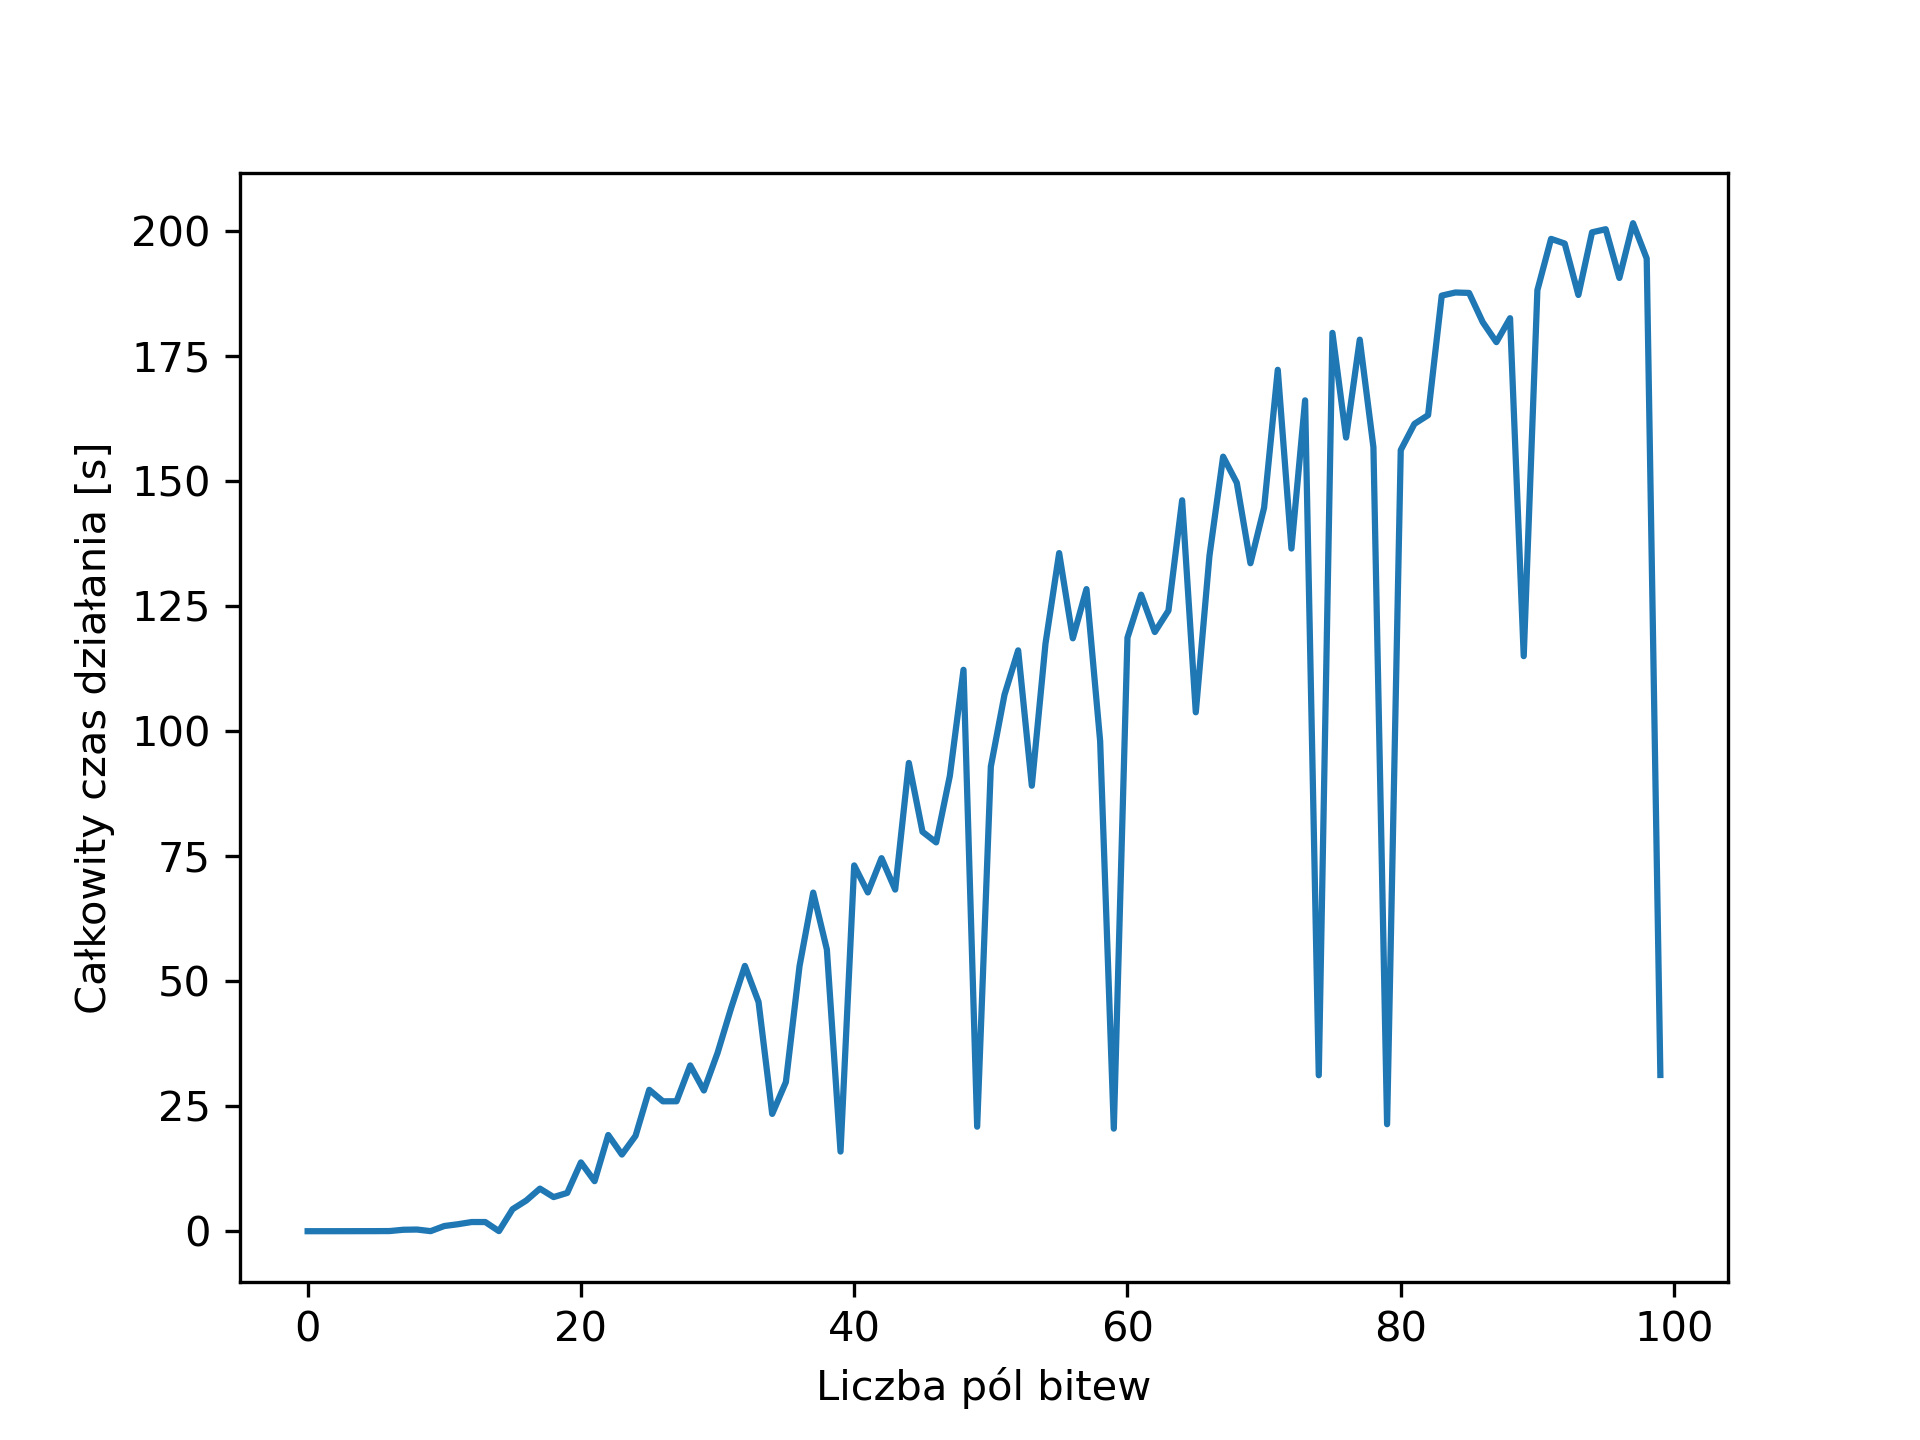
\includegraphics[width=360px]{./results/time_per_battlefields.png}
\end{center}

Na wykresie widać, że czasami algorytm jest dużo szybszy. Wynika to z tego, że
jego czas działania jest zależny od wielkości rozpatrywanych strategii.
Najczęściej z każdą iteracją algorytmu dodawana jest kolejna strategia czysta,
lecz w tych przypadkach algorytm po prostu znajduje równowagę, która jest mała.
Widać to na poniższym wykresie:

\begin{center}
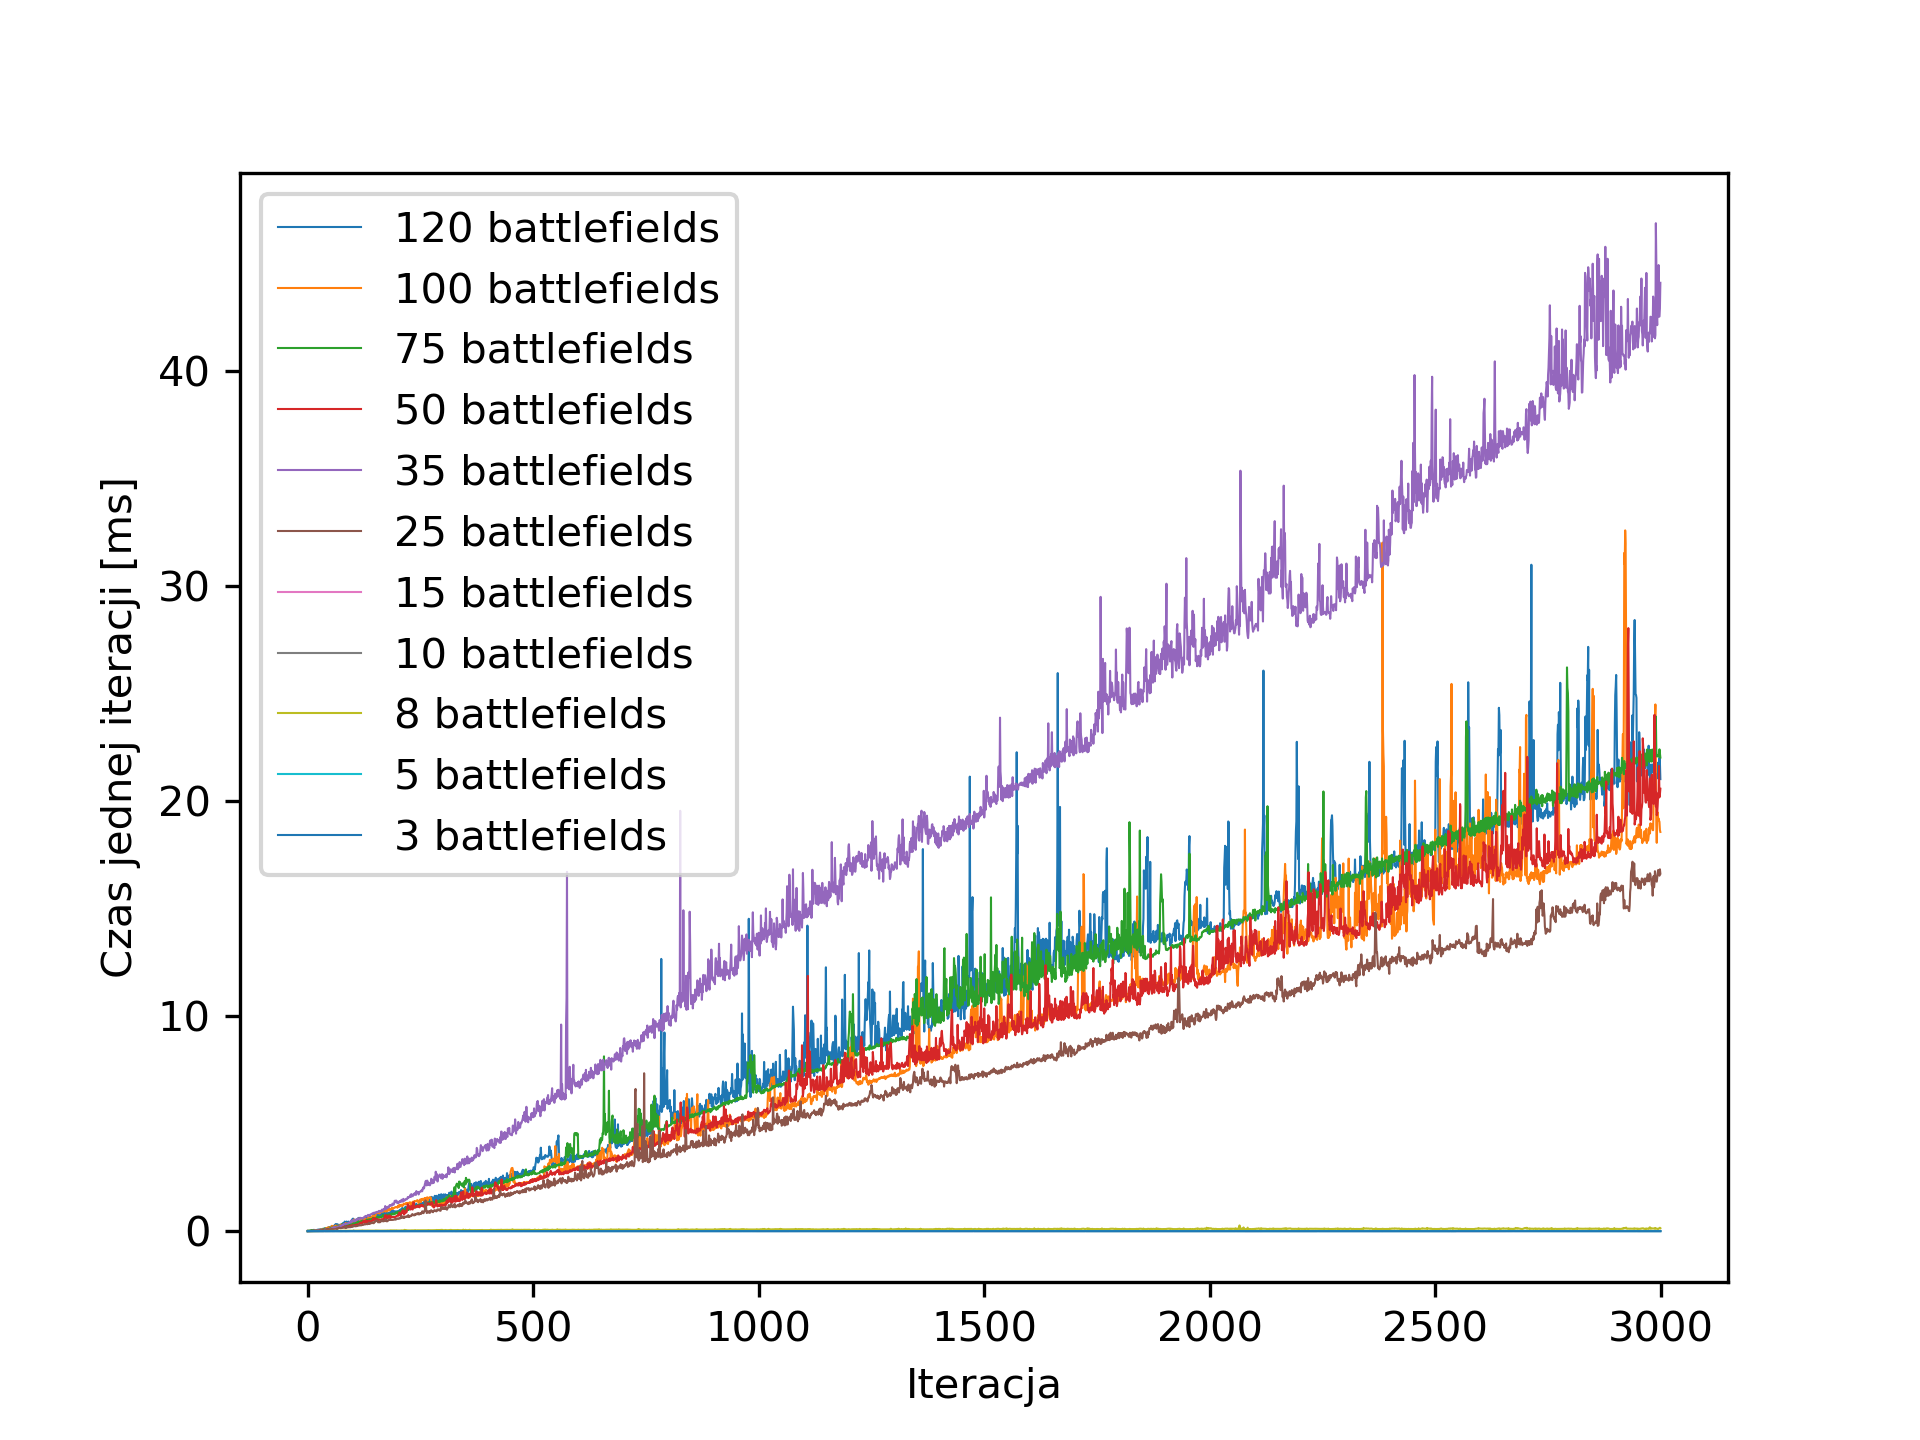
\includegraphics[width=360px]{./results/time_per_step.png}
\end{center}

W większości przypadków wykres czasu iteracji przypomina funkcję liniową, lecz
są przypadki, w którym jest to bardziej funkcja stała prawie równa 0.

\section{Analiza otrzymanego przybliżenia względem iteracji}

Algorytm uruchomiono na podzbiorze testów z poprzedniego punktu, ale na
zwiększonej liczbie iteracji.

Wykres został podzielony na dwie części -- pierwsze 50 iteracji oraz pozostałe.
\begin{center}
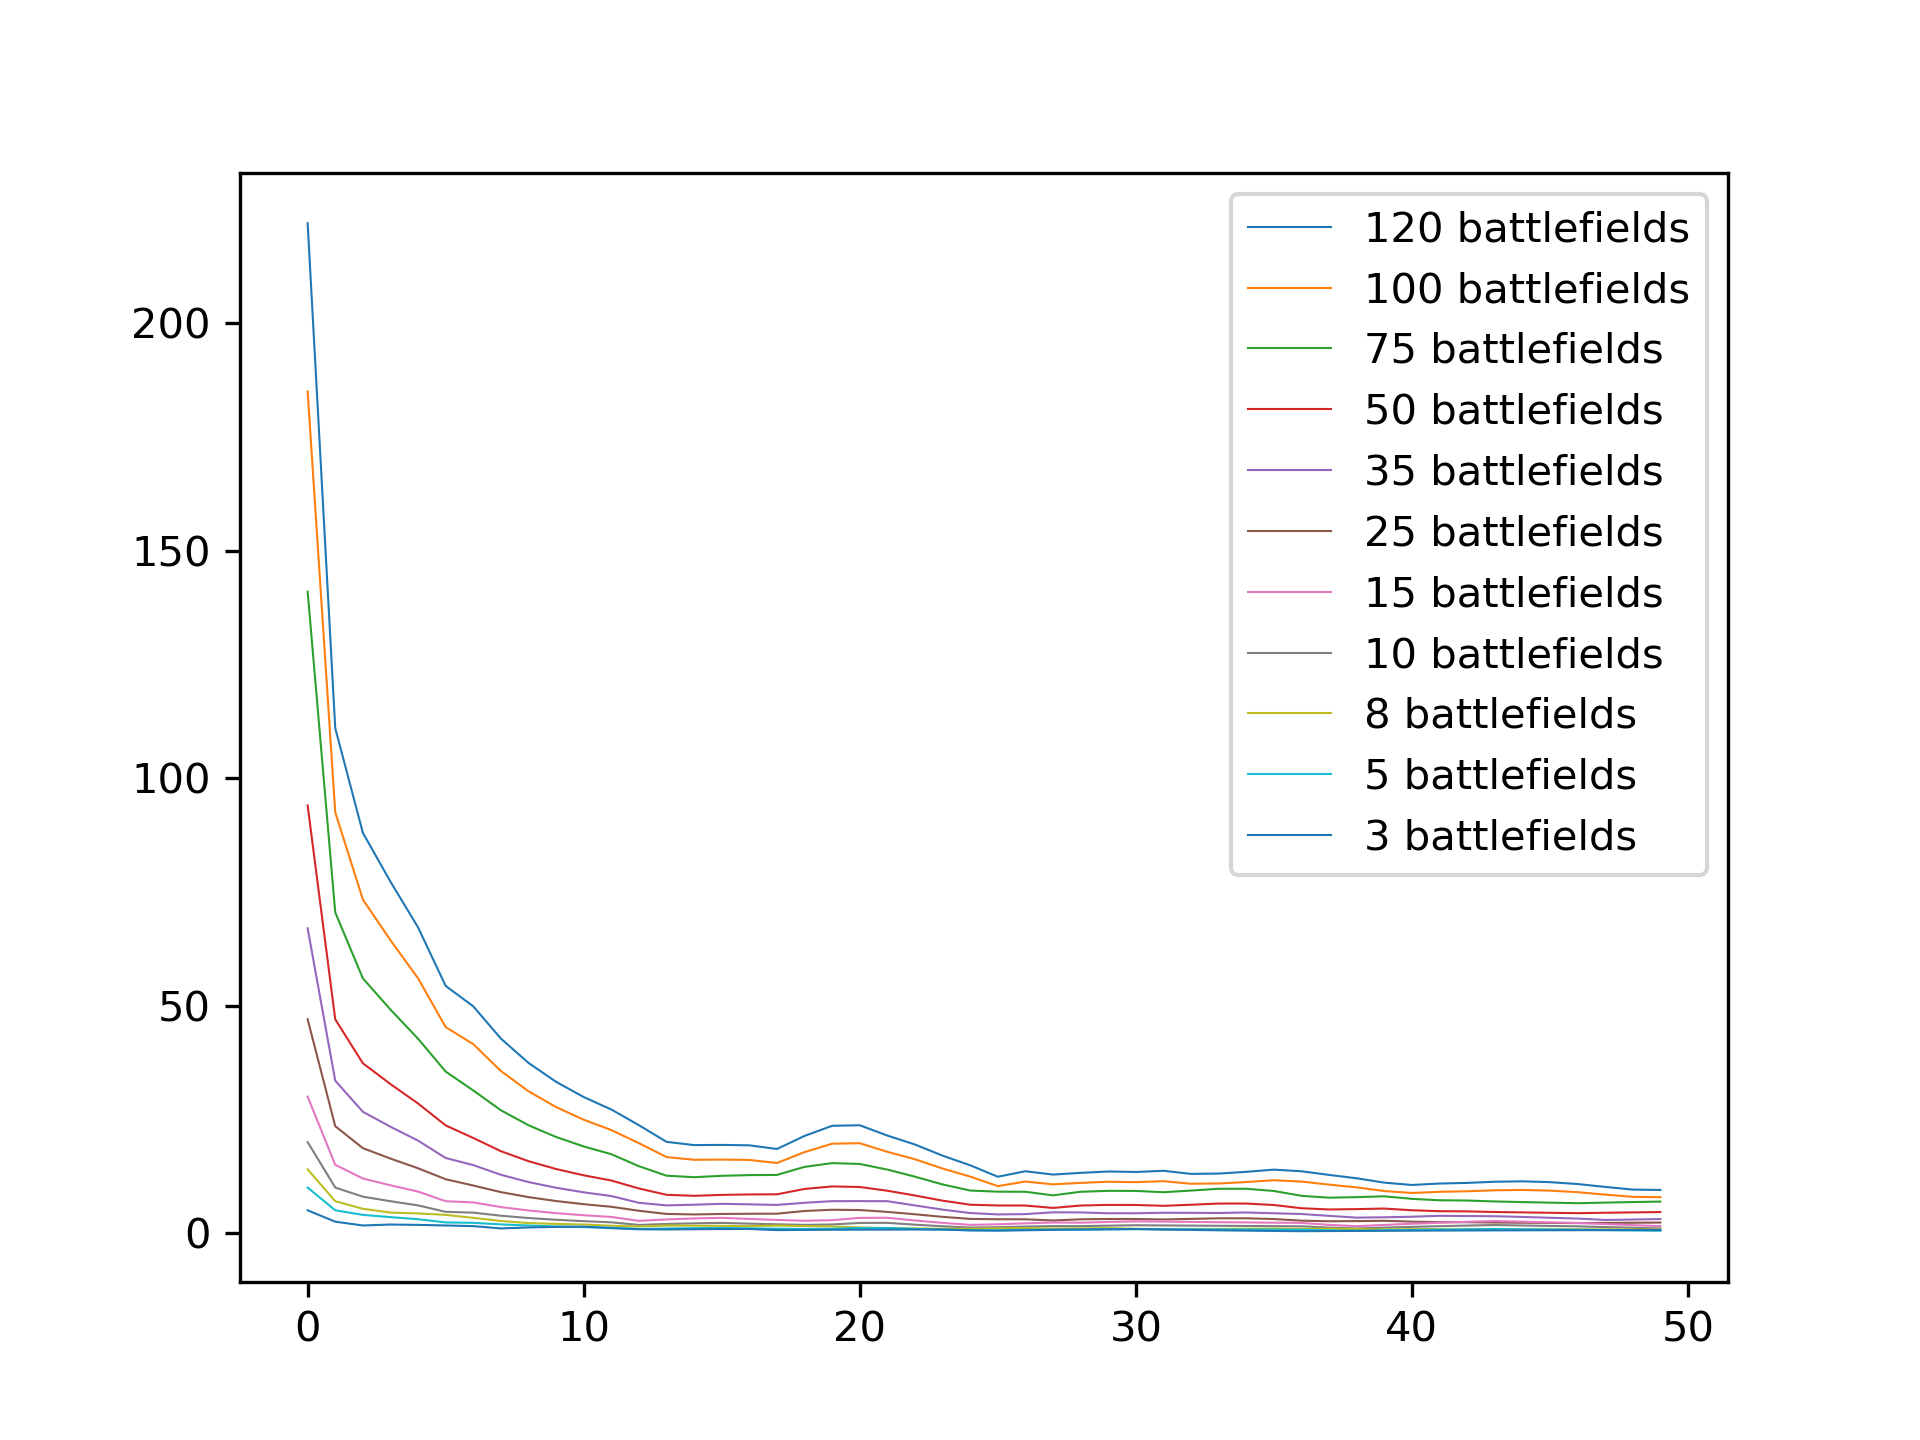
\includegraphics[width=360px]{./results/early_epsilon_after_step.png}

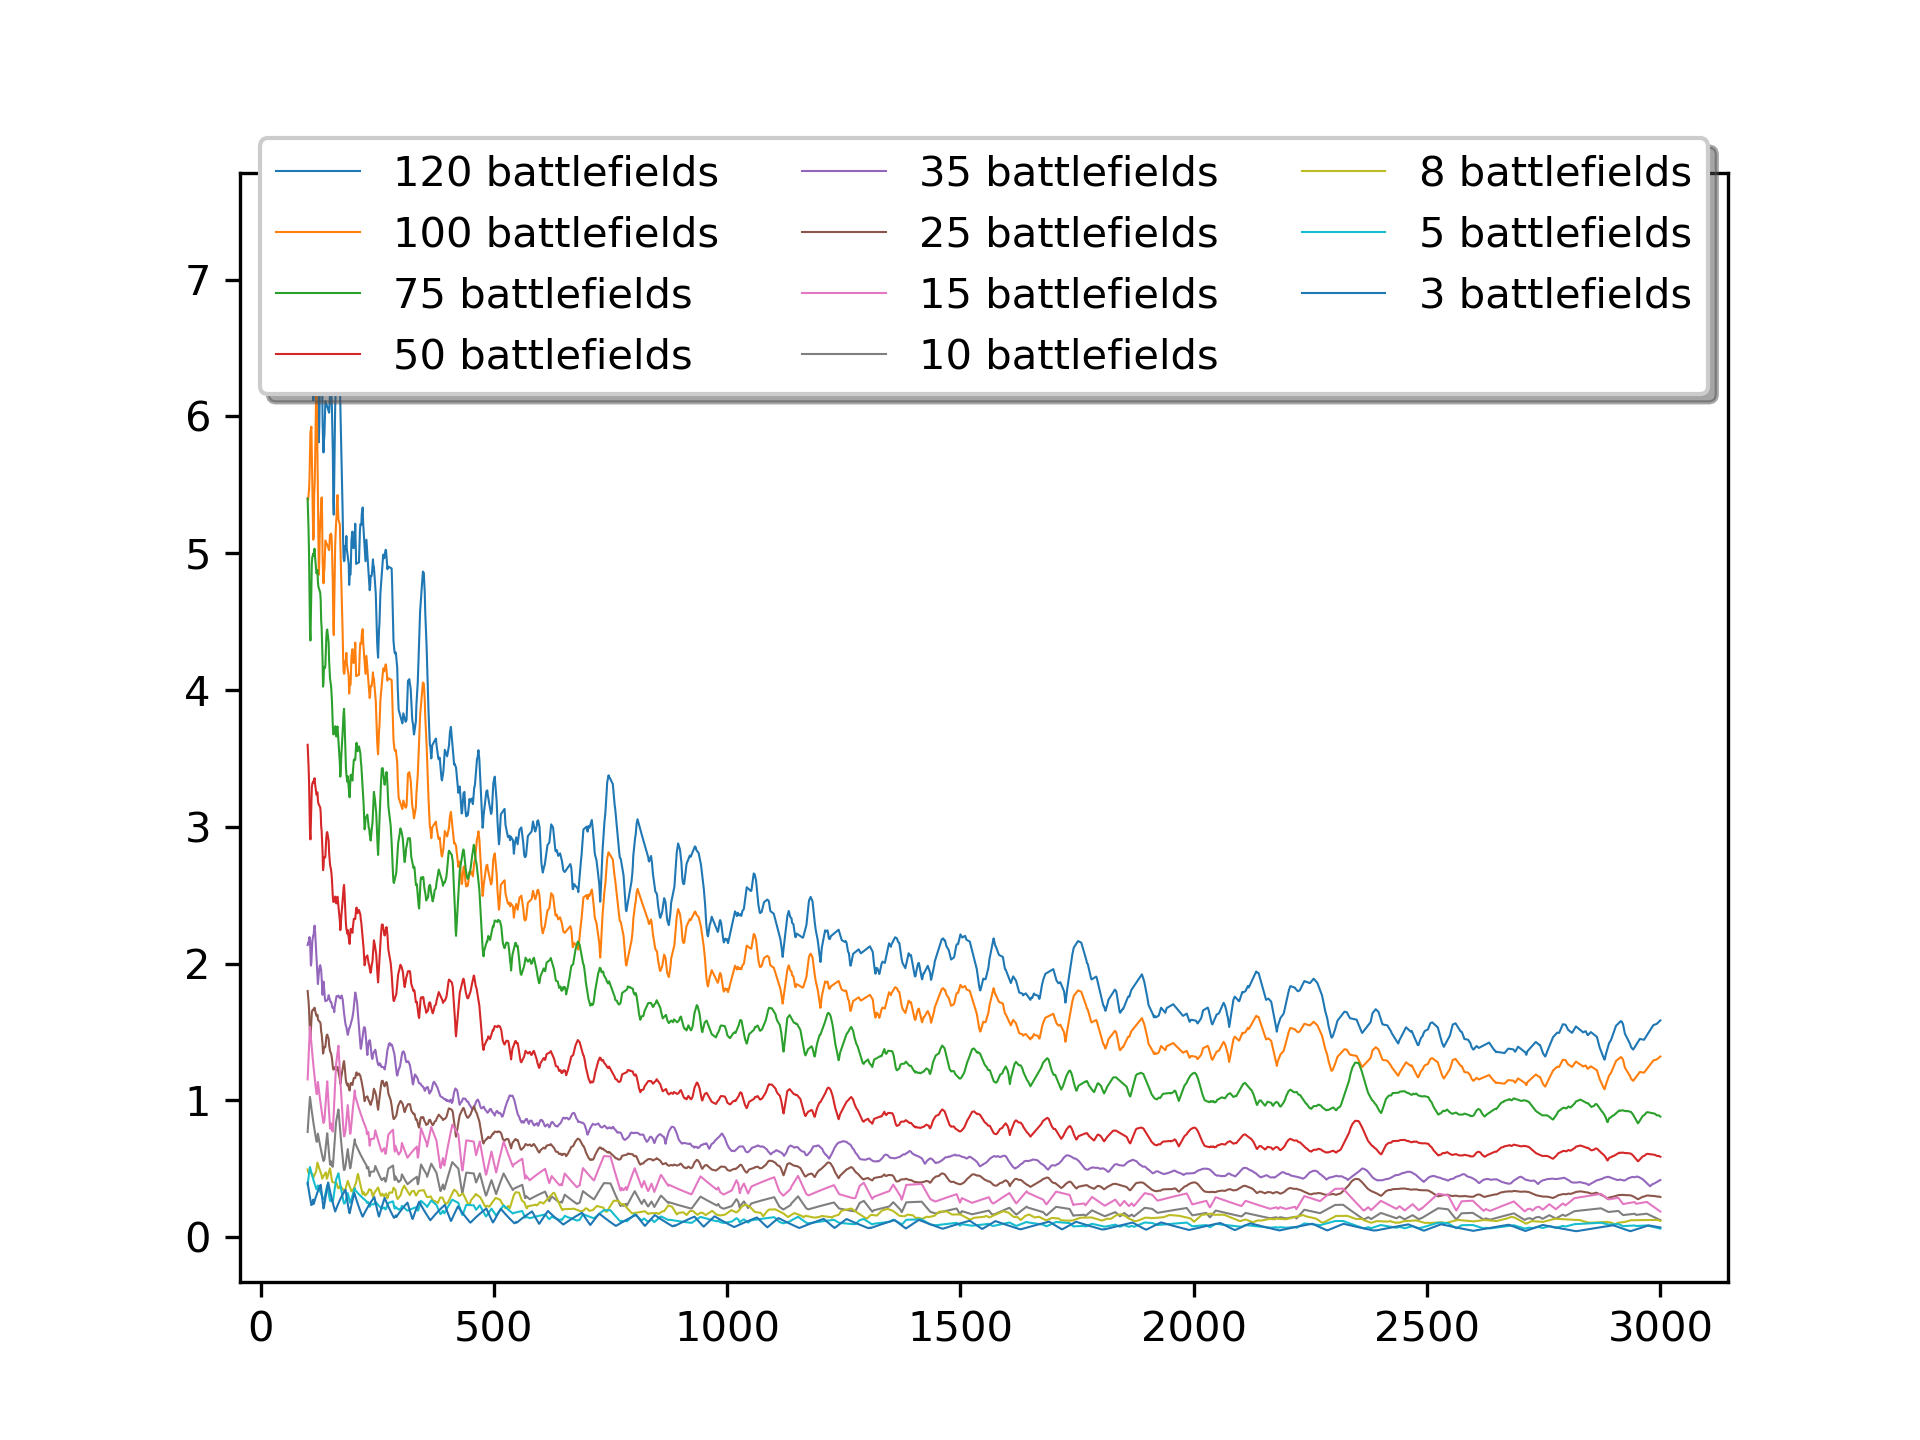
\includegraphics[width=360px]{./results/late_epsilon_after_step.png}
\end{center}

Na (drugim) wykresie ewidentnie widać pewne ograniczenie dolne zależne od
liczby iteracji, którego algorytm nigdy nie przebija.

\section{Analiza otrzymanego przybliżenia względem różnych strategii początkowych}

Algorytm uruchomiono na instancji z jednym polem wartości 2, dwoma polami
wartości 3, trzema polami wartości 4 oraz czterema polami wartości 5. Atakujący
miał 4 jednostki, a obrońca 7.

Strategiami graczy były: strategia jednorodna, atak / obrona najmniejszych pól,
atak / obrona największych pól.

\begin{center}
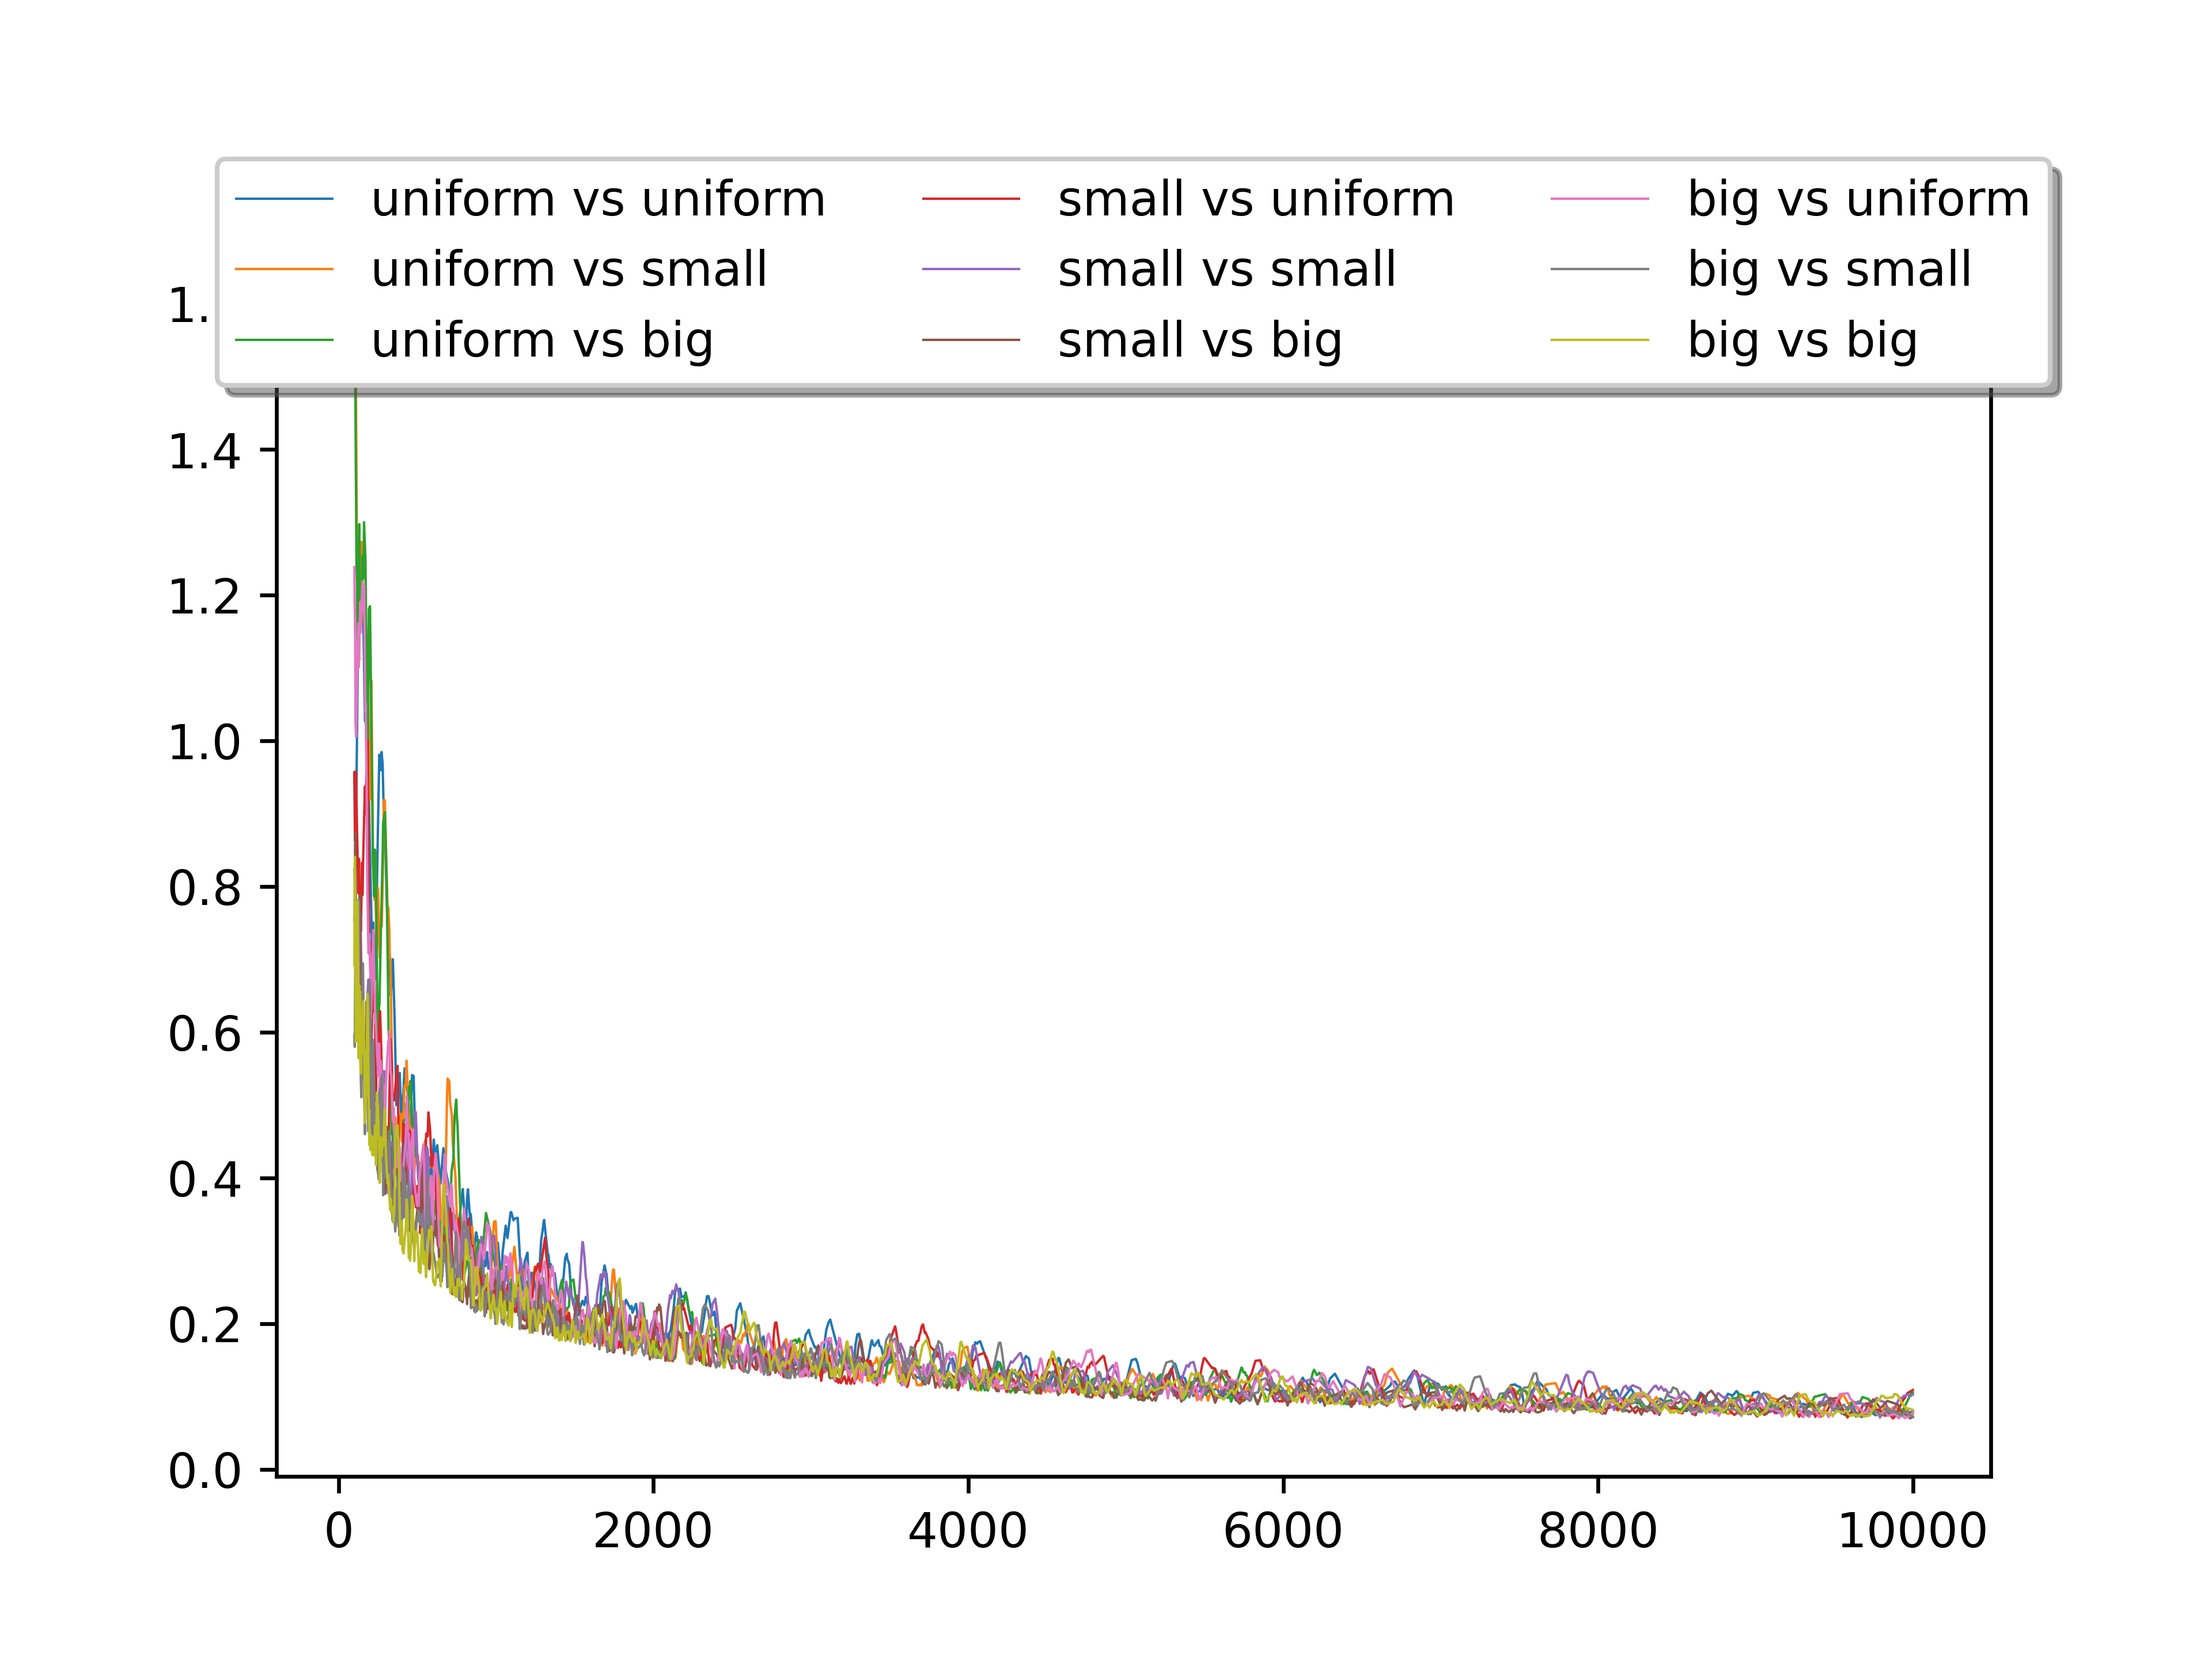
\includegraphics[width=360px]{./results/different_strats.png}
\end{center}

Nie zauważono istotnej różnicy w jakości przybliżenia ani szybkości zbiegania
w przypadku różnych strategii.

\section{Analiza otrzymanego przybliżenia wartości gry}

Z definicji gry, atakujący zawsze ma nieujemny wynik, a zatem obrońca ma wynik
niedodatni. Aby w równowadze wynik obrońcy był nieujemny (czyli tak właściwie
zerowy), musiałby on bronić wszystkich pól, czyli $BD = n$ (co swoją drogą
jest zakazane w treści).

\end{document}
